

  \begin{frame}[t]{Referencia na základe globálnej polohy}
\begin{itemize}
  \item<1-> Úlohou je držať polohu na základe globálnych súradníc (GS) napr. GPS. Pri minimalistickom prevedení (po zmene súradníc!) môžeme priamo premeniť polohu na uhol
  \item<2-> Ako by vyzeral náš kaskádovaný riadiaci systém?
  \item<3-> Môže to tak priamo fungovať?
\end{itemize}

  \begin{onlyenv}<1>
  \begin{figure}
\centering
  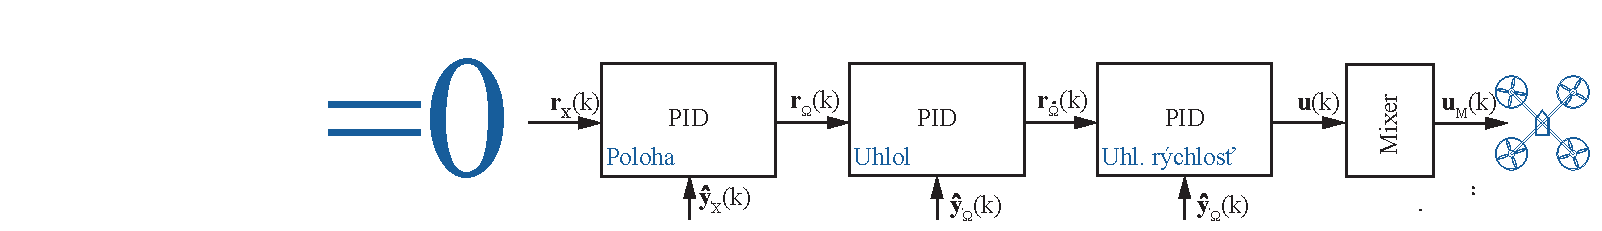
\includegraphics[width=\textwidth]{PID_HighLevel2a}\\
\end{figure}
\end{onlyenv}

  \begin{onlyenv}<2>
  \begin{figure}
\centering
  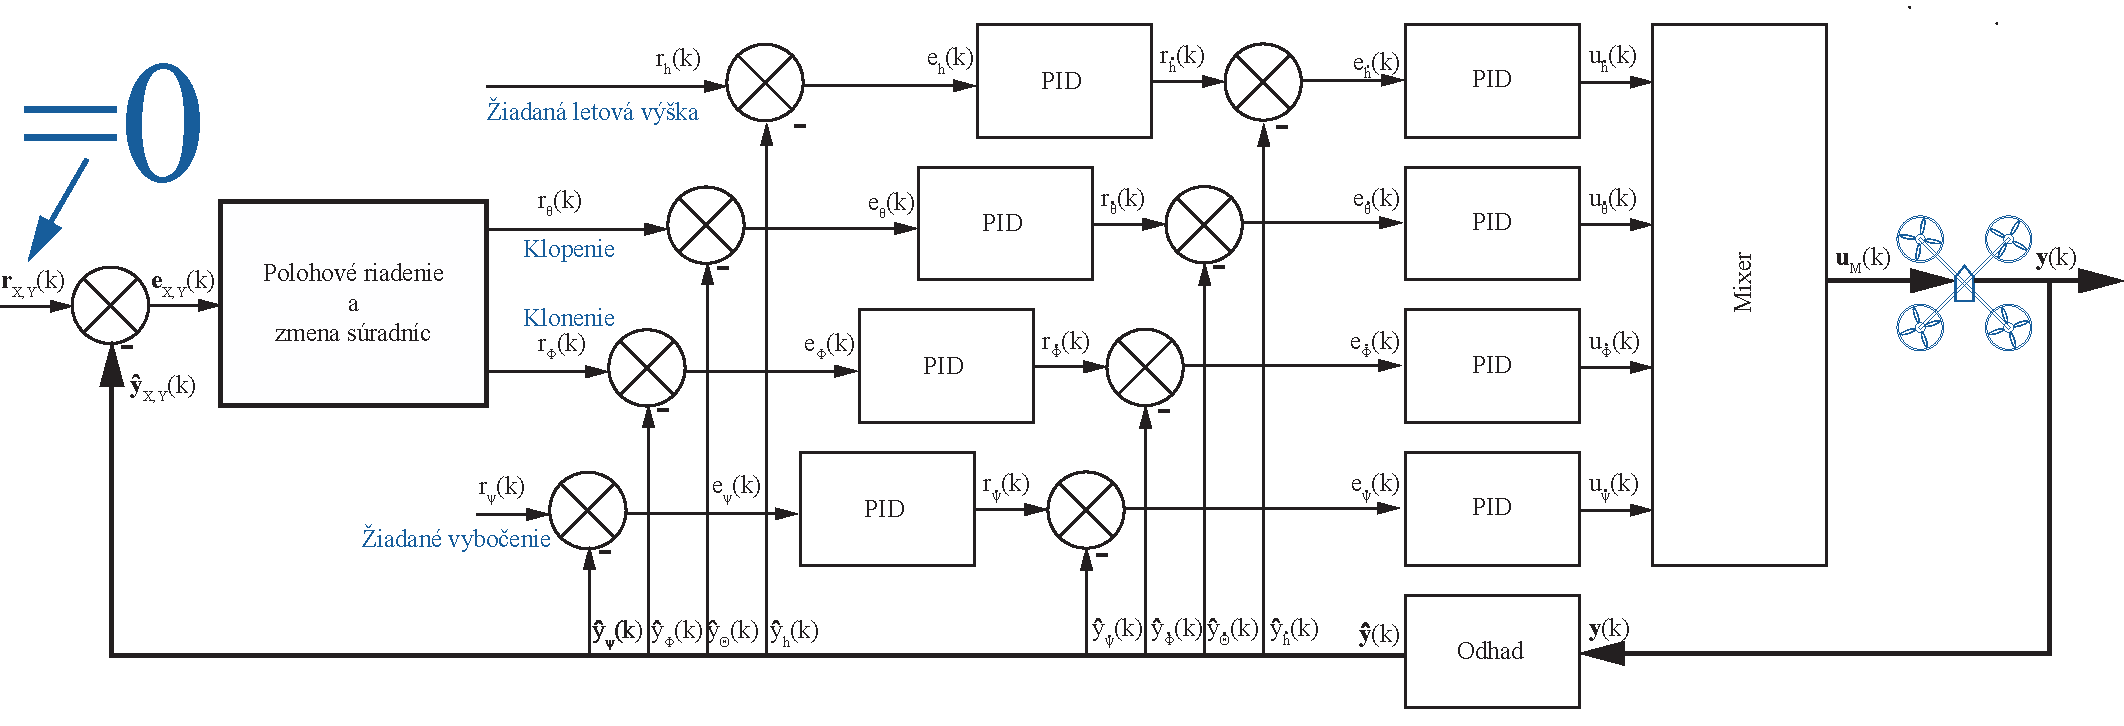
\includegraphics[width=\textwidth]{POS_Overall1}\\
\end{figure}
\end{onlyenv}

  \begin{onlyenv}<3>
  \begin{figure}
\centering
  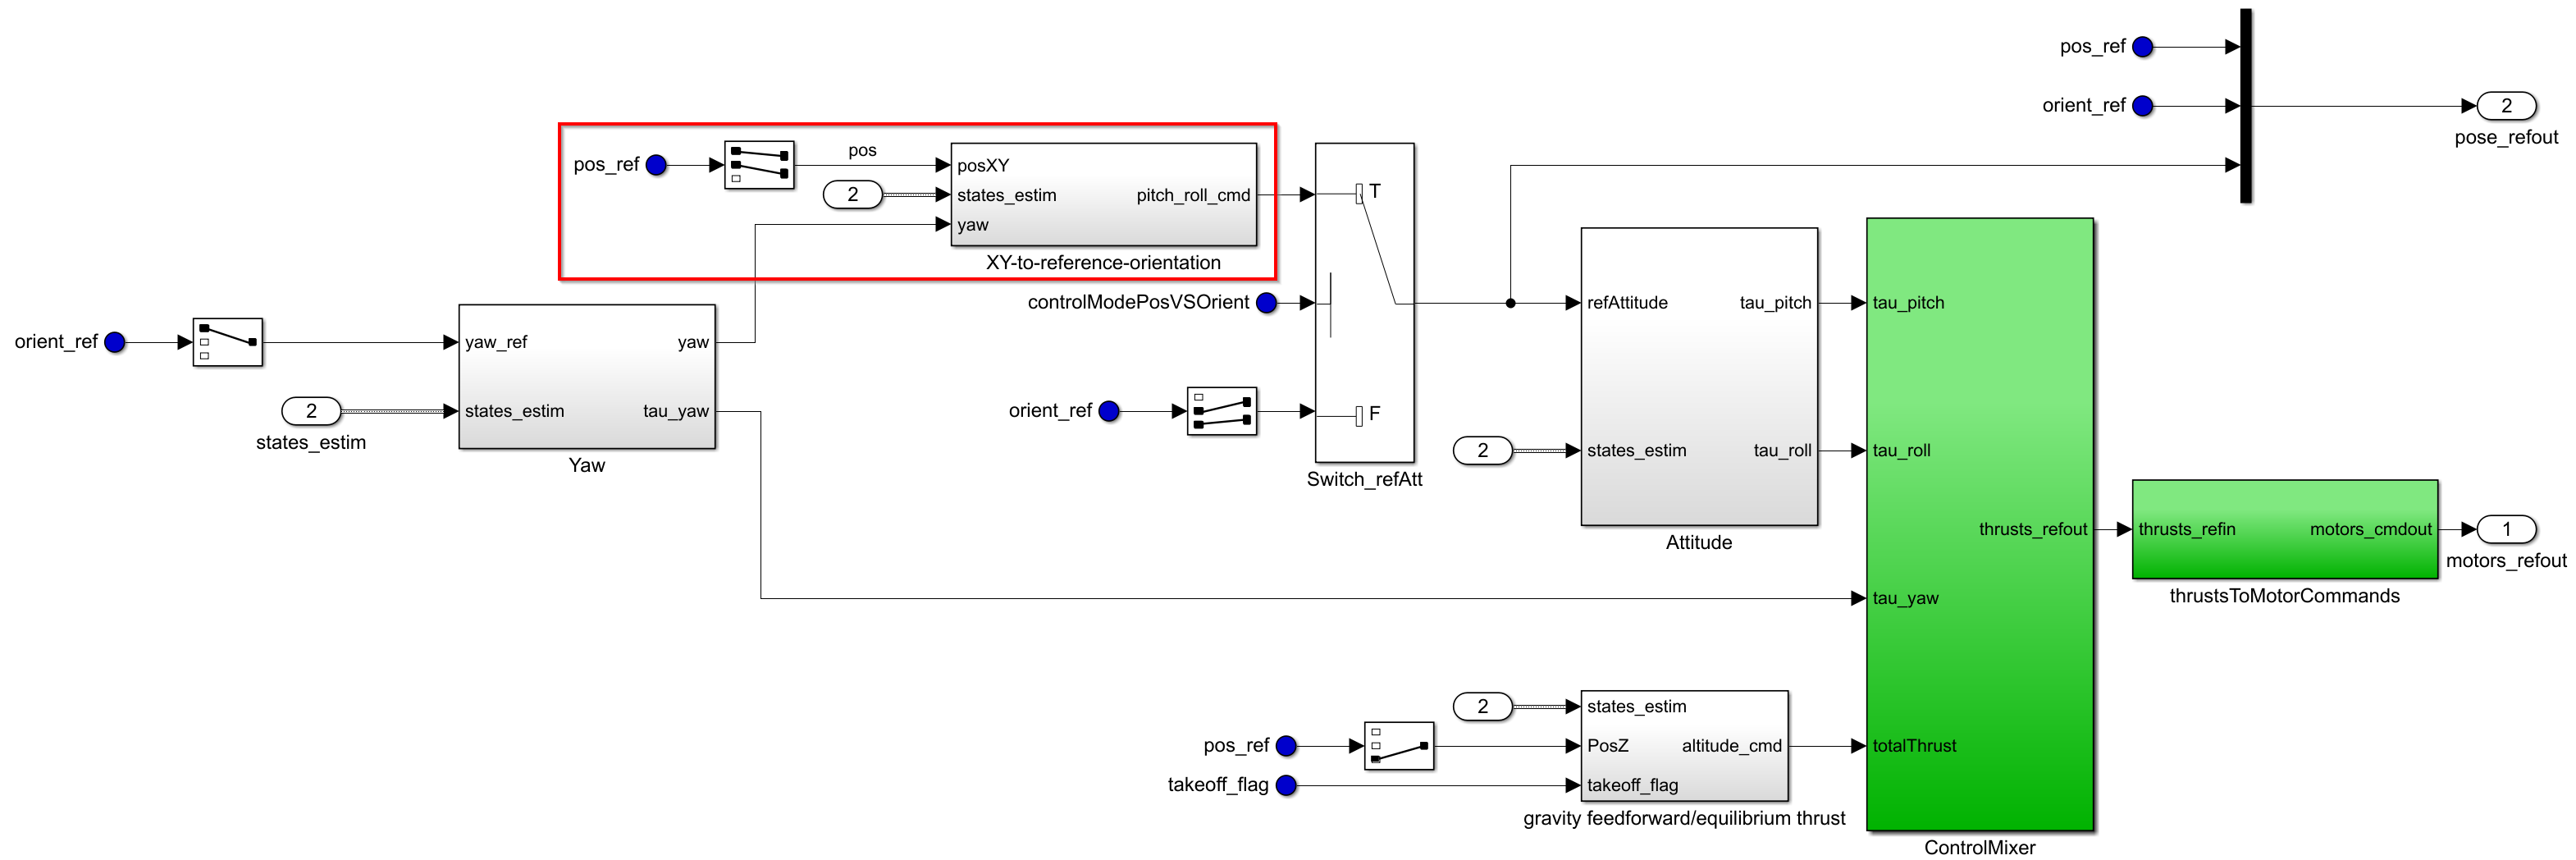
\includegraphics[width=\textwidth]{MS_QuadExample_Position1}\\
\end{figure}
\end{onlyenv}
\end{frame}


 \begin{frame}[t]{Zmena súradníc}
\begin{itemize}
  \item<1-> Aj pri priamom riadení polohy musíme zmeniť súradnice
  \item<2-> Klopenie a klonenie určíme na základe GS súradníc, t.j. premeníme $X,Y\rightarrow\Theta,\Phi$...
  \item<3->  ...   ale potrebujeme na výpočet aj želané/aktuálne vybočenie, t.j. $X,Y,\Psi\rightarrow\Theta,\Phi$,
\end{itemize}

  \begin{onlyenv}<1>
  \begin{figure}
\centering
  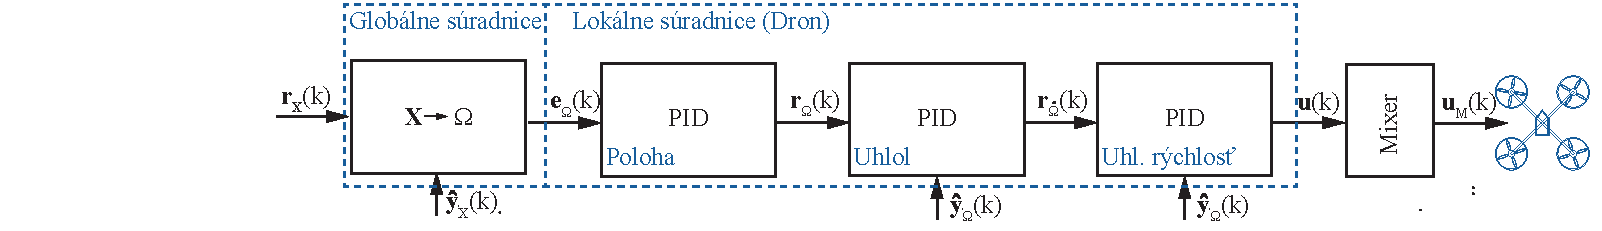
\includegraphics[width=\textwidth]{PID_HighLevel3a}\\
\end{figure}
\end{onlyenv}

  \begin{onlyenv}<2>
  \begin{figure}
\centering
  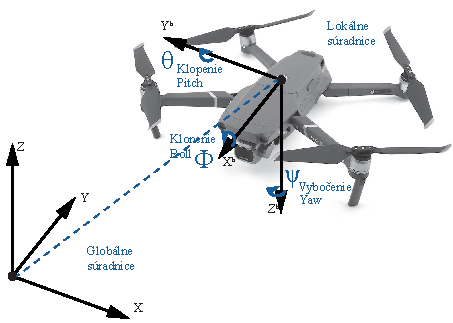
\includegraphics[width=70mm]{rollpitch2}\\
\end{figure}
\end{onlyenv}


  \begin{onlyenv}<3>
  \begin{figure}
\centering
  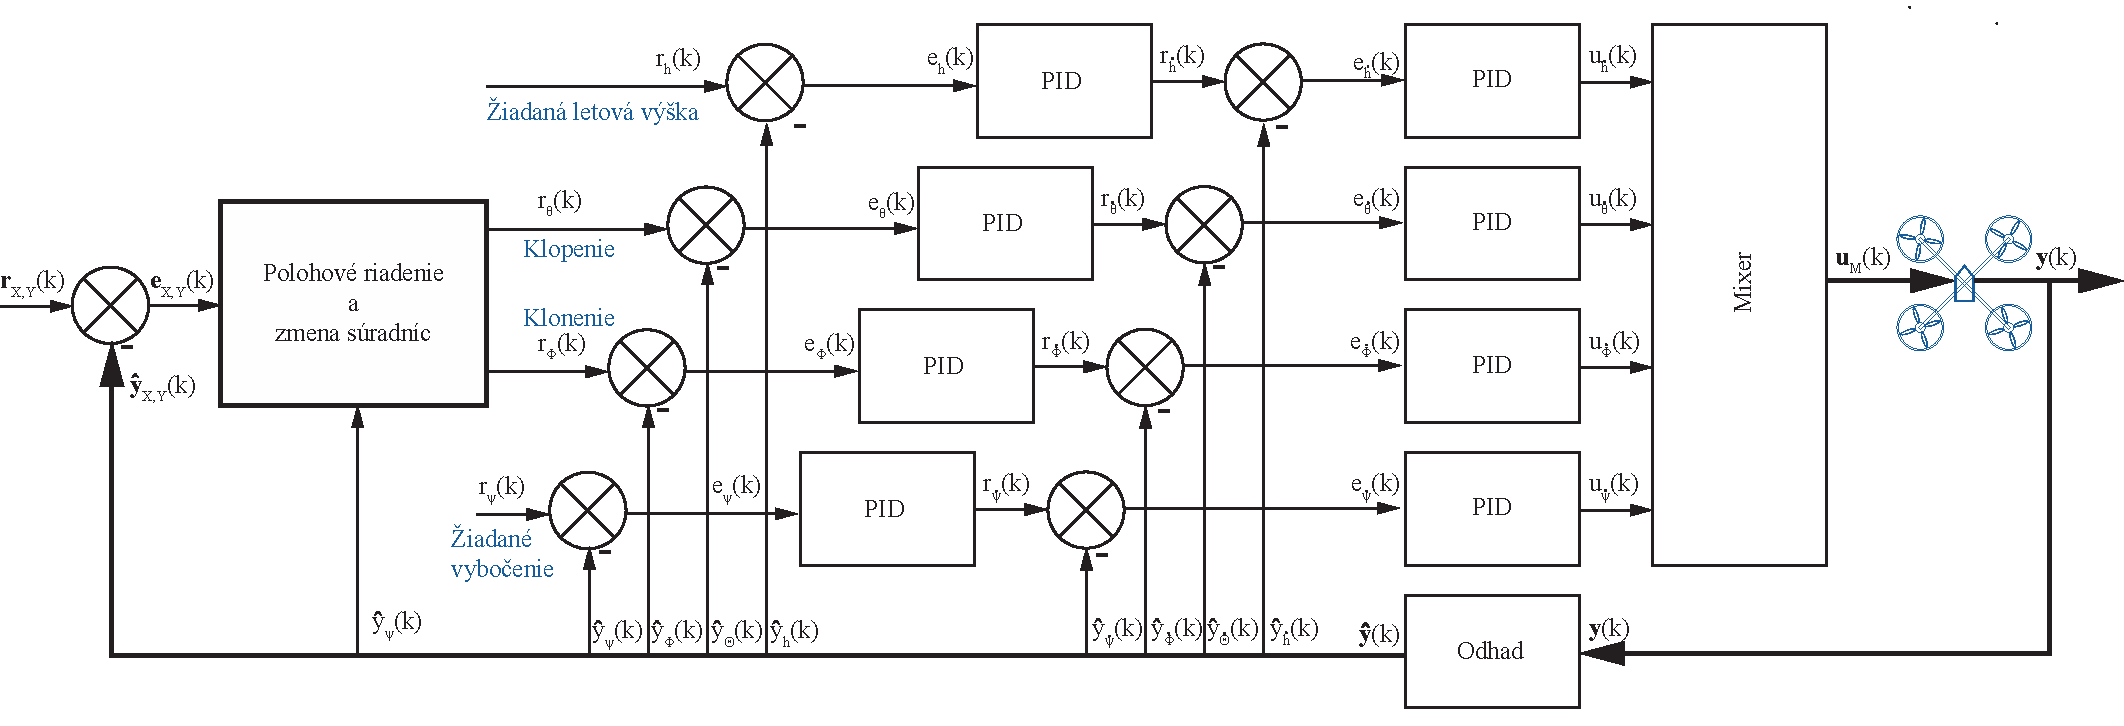
\includegraphics[width=\textwidth]{POS_Overall2}\\
\end{figure}
\end{onlyenv}
\end{frame}

 \begin{frame}[t]{Zmena súradníc 2}
\begin{itemize}
  \item<1-> Môžeme napr. používať trigonometriu, teda rotačné matice \angl{direction cosine matrix, DCM} na premenu z globálnych (G) do lokálnych (L) súradníc
  \item<2-> Najjednoduchší ale funkčný príklad, stabilizácia klonenia a klopenia. Majme odchýlku polohy $\vec{e}^{\mathbf{G}}_{X,Y}=\begin{bmatrix}X,Y\end{bmatrix}^T$ a aktuálne vybočenie $\Psi$, potom \citep{BenAri2017}
      \begin{align}
      \vec{e}^{\mathbf{L}}_{\Theta,\Phi}=
      \begin{bmatrix}
          \cos{\Psi} & -\sin{\Psi} \\
          \sin{\Psi} & \cos{\Psi}
      \end{bmatrix}
      \vec{e}^{\mathbf{G}}_{X,Y}
      \end{align}
  \item<3-> V príklade v MATLAB/Simulink je to prakticky identické
\end{itemize}

  \begin{onlyenv}<3>
  \begin{figure}
\centering
  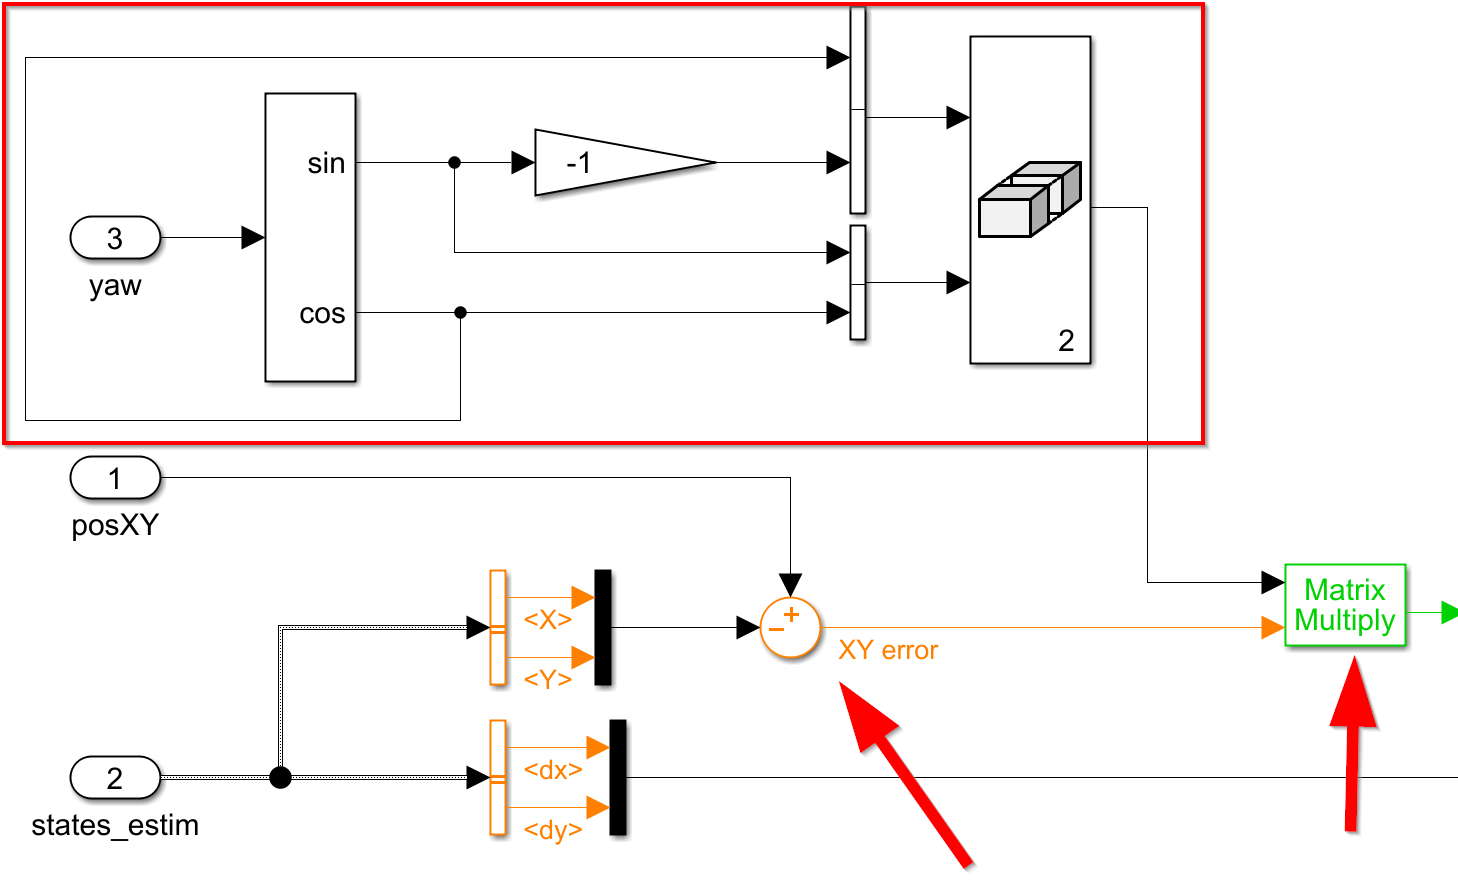
\includegraphics[width=50mm]{MS_QuadExample_Position2}\\
\end{figure}
\end{onlyenv}

\end{frame}


 \begin{frame}[t]{Zmena súradníc 3}
\begin{itemize}
  \item<1-> ArduCopter využíval DCM až do v. 3.2.  
   \item<2-> Pri 3D reprezentácii DCM sa začínajú komplikovať, a obsahujú singularity \citep{BenAri2017}
   \item<3-> Riešenie: reprezentácia Eulerových uhlov cez kvaternióny \angl{quaternion} ktoré odstránia problém so singularitou a sú výpočtovo efektívnejšie \citep{BenAri2017}
       \item<4-> V súčasných verziách aj ArduCopter aj PX4 využíva kvaternióny
\end{itemize}
\end{frame}



\begin{frame}{Priame riadenie polohy}

  \begin{onlyenv}<1>
  \begin{figure}
\centering
  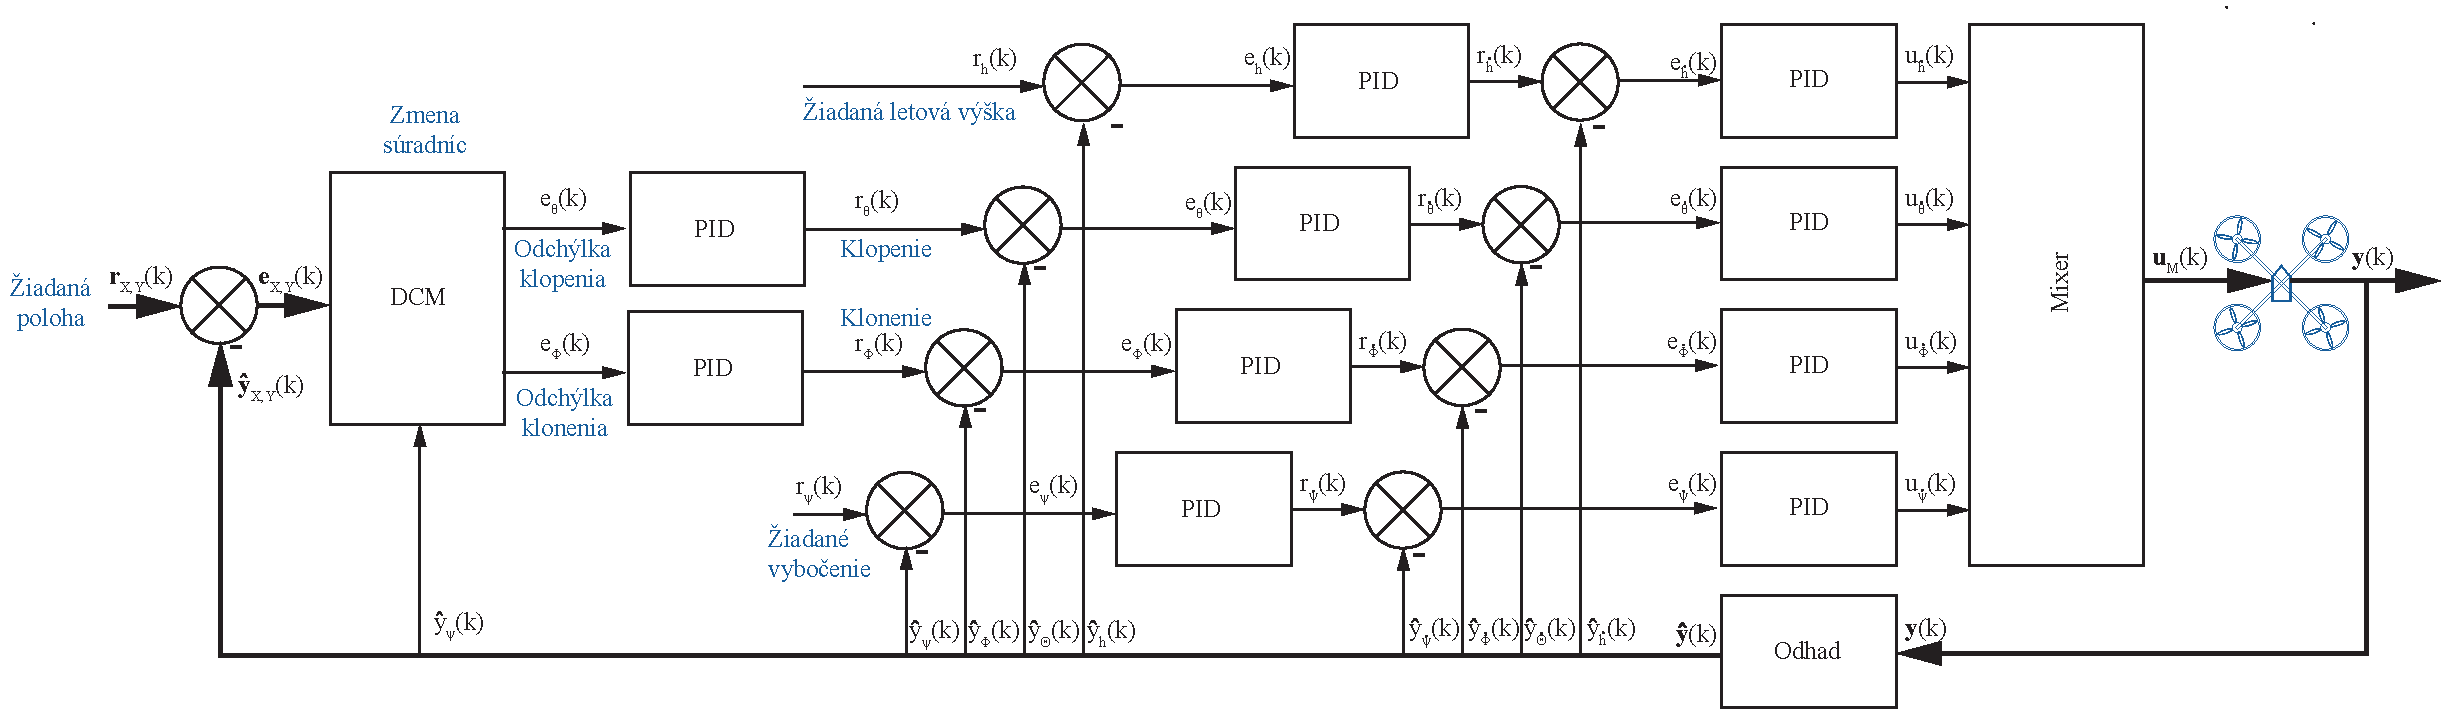
\includegraphics[width=\textwidth]{POS_Overall3}\\
\end{figure}
\end{onlyenv}


  \begin{onlyenv}<2>
  \begin{figure}
\centering
  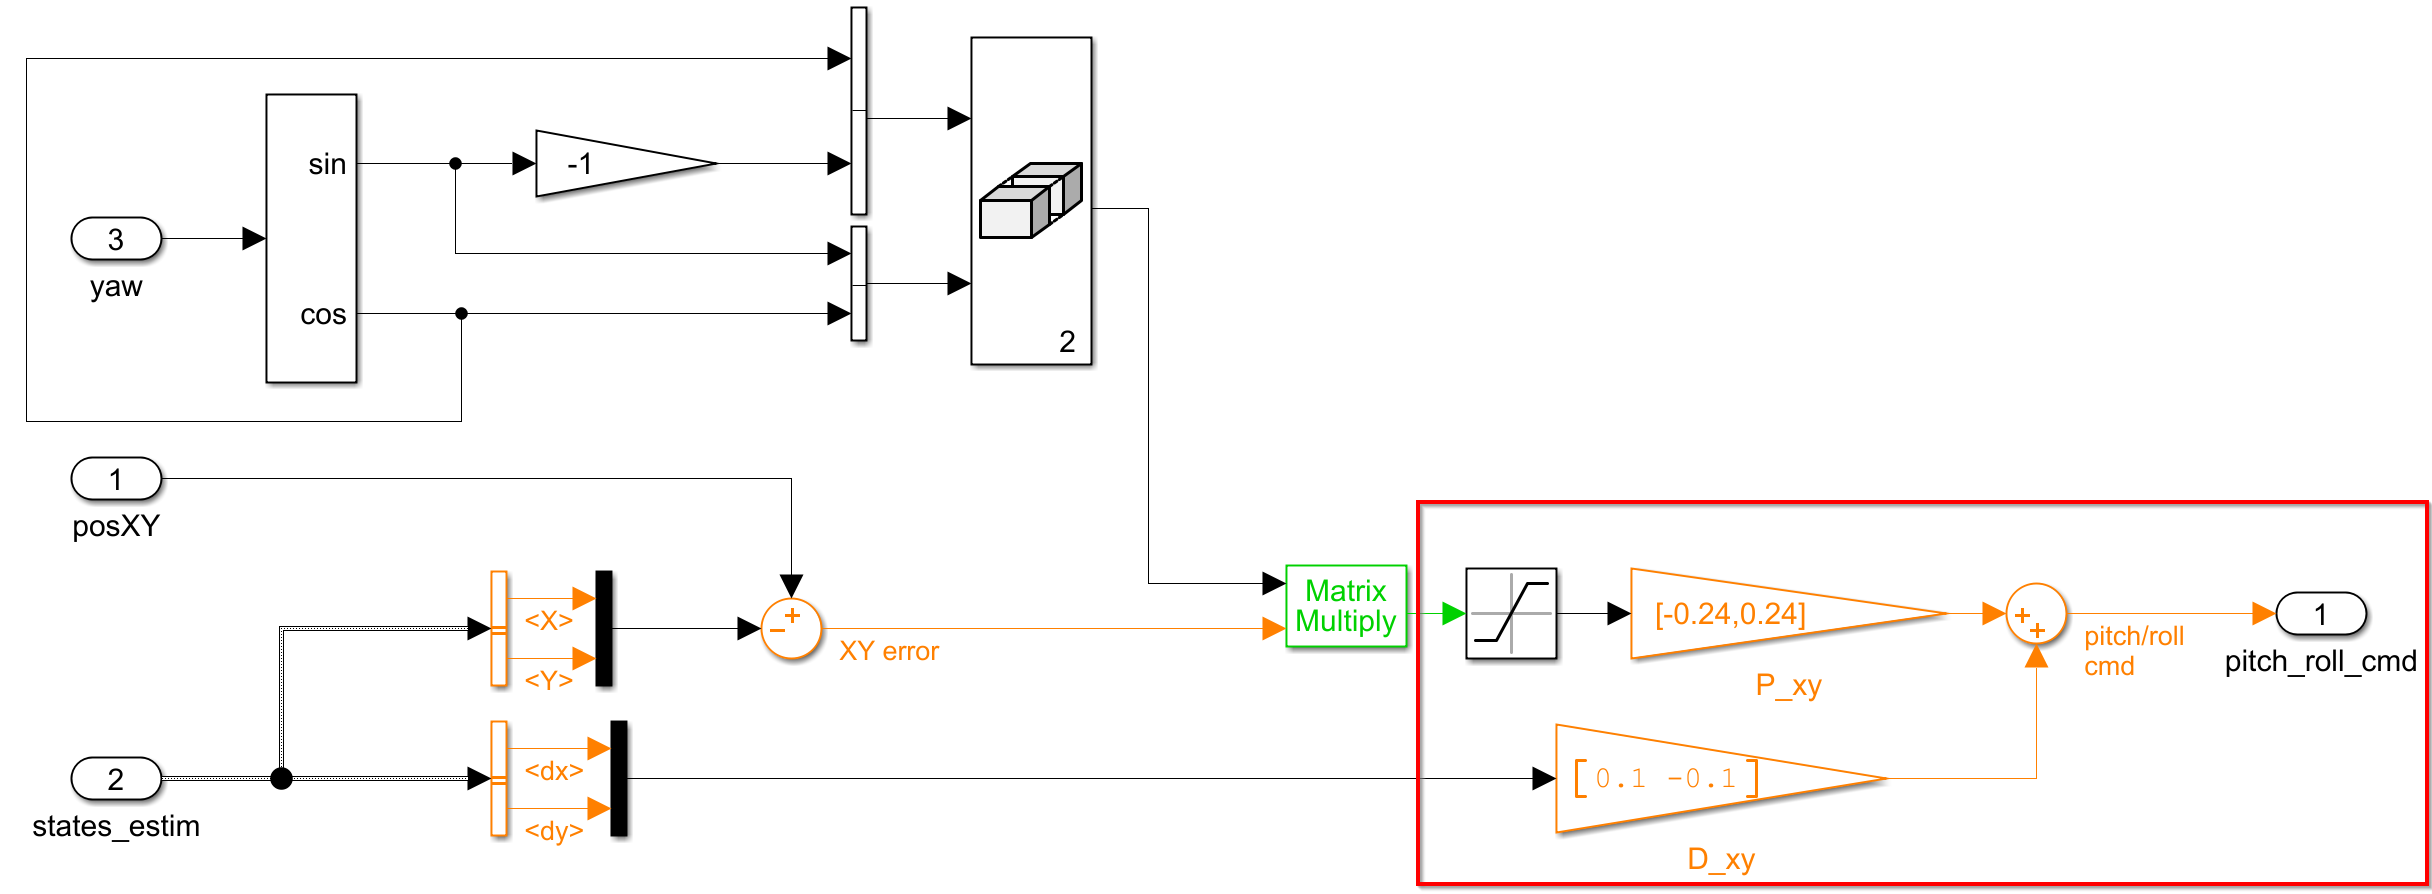
\includegraphics[width=\textwidth]{MS_QuadExample_Position3}\\
\end{figure}
\end{onlyenv}
\end{frame}




%---------------------Zmena suradnic inde----------------
%  \begin{frame}[t]{Zmena súradníc}
%\begin{itemize}
%  \item<1-> aaaa
%\end{itemize}
%  \begin{onlyenv}<1>
%  \begin{figure}
%\centering
%  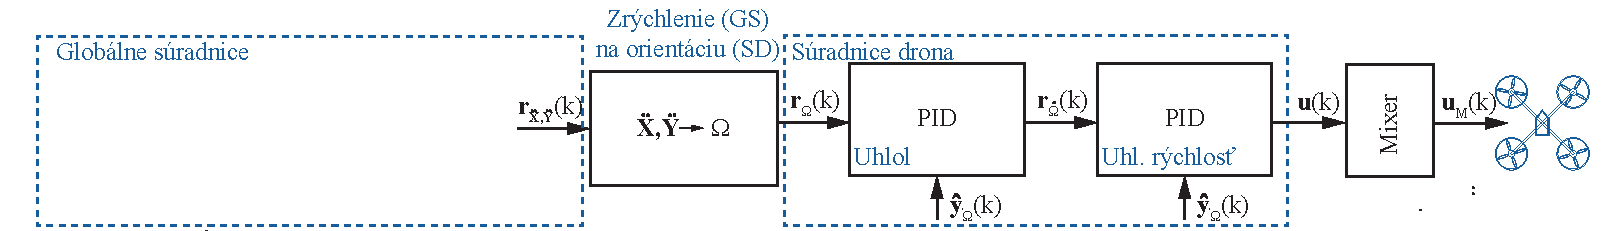
\includegraphics[width=\textwidth]{PID_HighLevel2}\\
%\end{figure}
%\end{onlyenv}

  \begin{frame}[t]{Nepriame riadenie polohy: Riadenie rýchlosti}
\begin{itemize}
\item<1-> V skutočnosti aby sme vedeli korigovať aj polohu aj rýchlosť na základe odhadov, aj tu máme ďalšie kaskádové prevedenie. Pridáme tzv. rýchlostnú slučku
\item<2-> Transformácia súradníc je logicky na inom mieste
\item<3-> Namiesto $X,Y\rightarrow\Theta,\Phi$ máme $X,Y\rightarrow \dot{X},\dot{Y}\rightarrow \ddot{X},\dot{Y}\rightarrow\Theta,\Phi$
\item<4->  Väčšinou je to plné PID riadenie, ako aj pri ArduCopter, PX4 a inde (c.f. \cite{Saha2020}).
\end{itemize}

  \begin{onlyenv}<2>
  \begin{figure}
\centering
  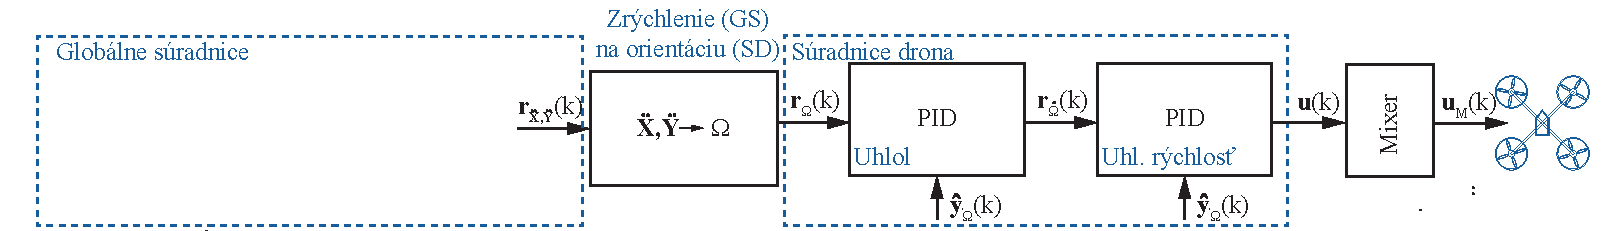
\includegraphics[width=\textwidth]{PID_HighLevel2}\\
\end{figure}
\end{onlyenv}


  \begin{onlyenv}<3>
  \begin{figure}
\centering
  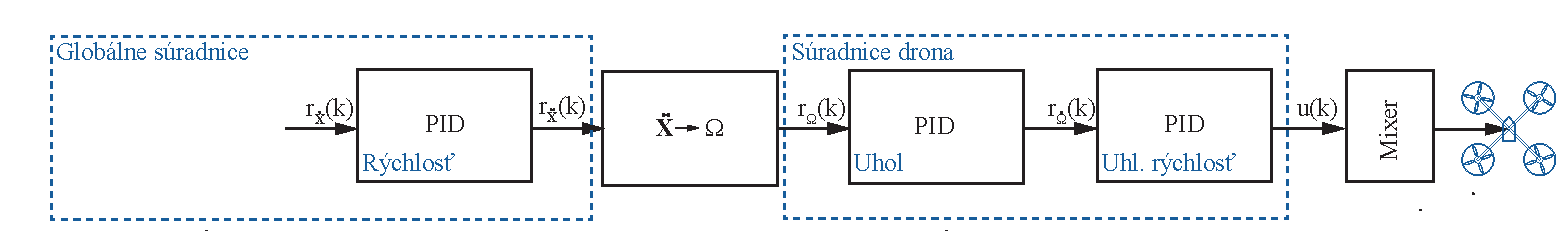
\includegraphics[width=\textwidth]{PID_HighLevel3}\\
\end{figure}
\end{onlyenv}


  \begin{onlyenv}<4>
  \begin{figure}
\centering
  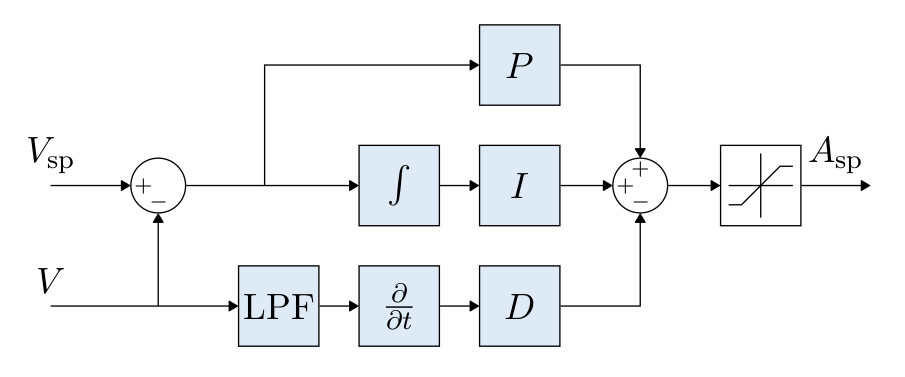
\includegraphics[width=70mm]{PX4_Velocity}\\
\end{figure}
\end{onlyenv}
  \end{frame}


  
   \begin{frame}[t]{Nepriame riadenie polohy: Polohová slučka}
\begin{itemize}
  \item<1-> Potrebujeme ešte jednu slučku --- polohovú, ktorá premení polohu na rýchlosť

  \item<2-> Väčšinou je to P riadenie, ako aj pri ArduCopter, PX4 a inde (c.f. \cite{Saha2020}).
\end{itemize}

  \begin{onlyenv}<1->
  \begin{figure}
\centering
  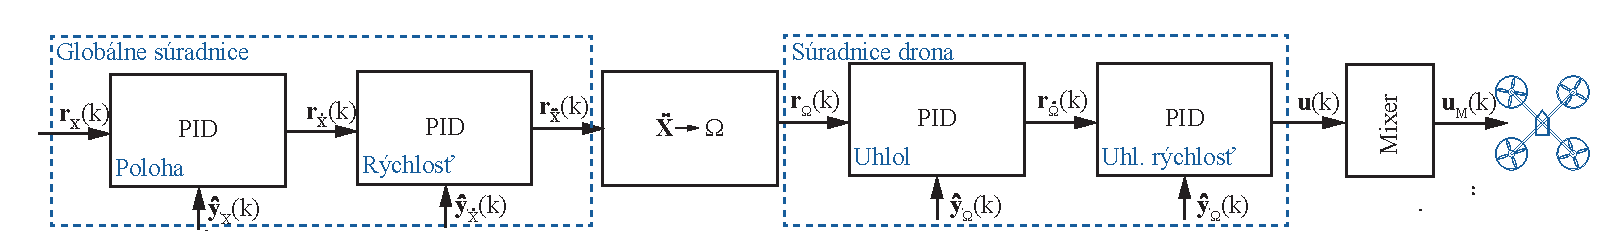
\includegraphics[width=\textwidth]{PID_HighLevel4}\\
\end{figure}
\end{onlyenv}


  \begin{onlyenv}<2->
  \begin{figure}
\centering
  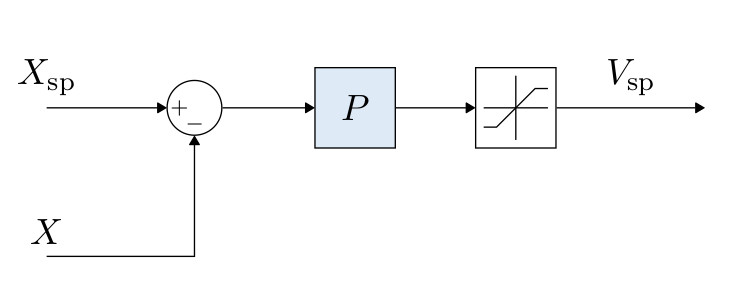
\includegraphics[width=50mm]{PX4_Position}\\
\end{figure}
\end{onlyenv}
  \end{frame}
  
 \begin{frame}[t]{Celková riadiaca architektúra}
  \begin{onlyenv}<1>
  \begin{figure}
\centering
  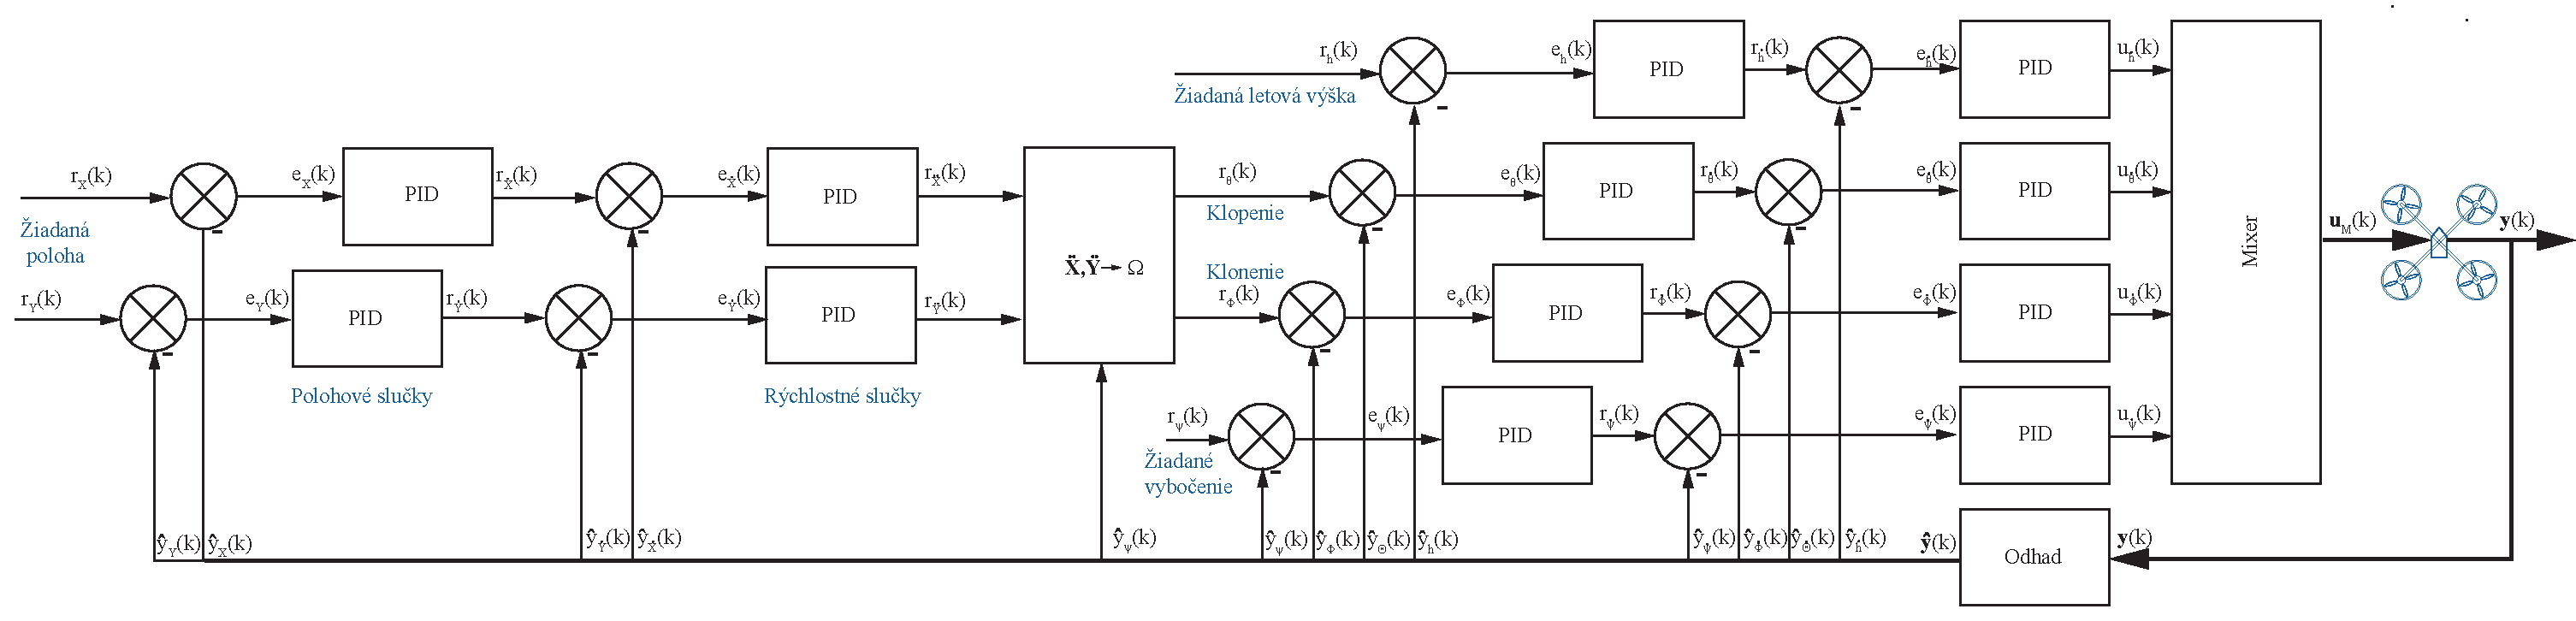
\includegraphics[width=\textwidth]{POS_Overall4}\\
\end{figure}
\end{onlyenv}

  \begin{onlyenv}<2>
  \begin{figure}
\centering
  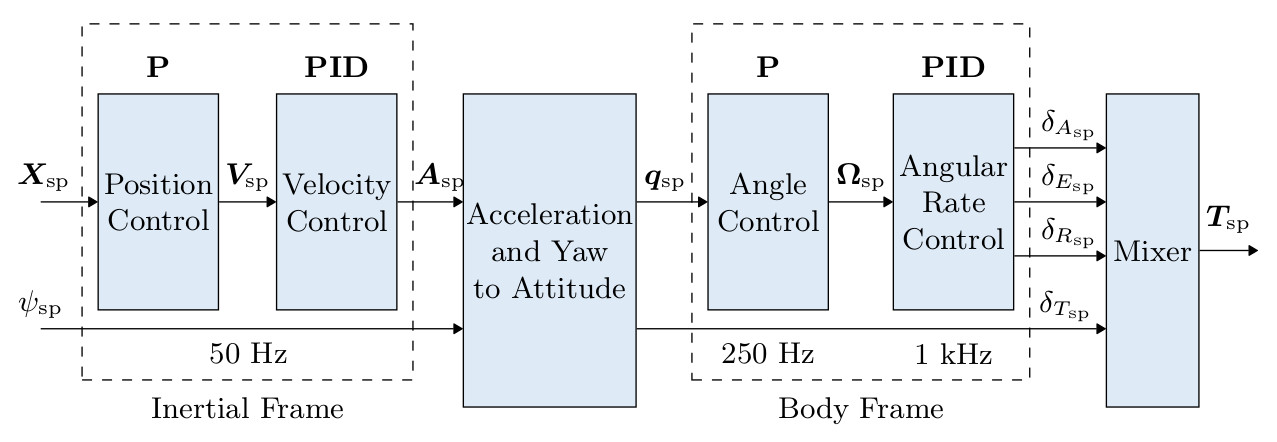
\includegraphics[width=\textwidth]{PX_Overall}\\
\end{figure}
\end{onlyenv}

  \end{frame}
  
  

\begin{frame}{Je dokonalé sledovanie trasy vôbec možné?}
\begin{itemize}
\item<1-> Majme trasu WP1 do WP2, všetko je v poriadku.
\item<2-> Pridajme WP3 a rozmýšľajme čo sa deje pri WP2. Je možné preletieť nad WP2?
\item<3-> Buď musíme úplne sa zastaviť alebo nemôžeme priamo preletieť --- ináč by sme potrebovali nekonečne veľké zrýchlenia
\end{itemize}

\begin{onlyenv}<1>
  \begin{figure}
\centering
  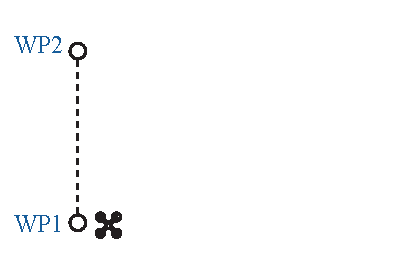
\includegraphics[width=60mm]{PositionControl}\\
\end{figure}
\end{onlyenv}

\begin{onlyenv}<2>
  \begin{figure}
\centering
  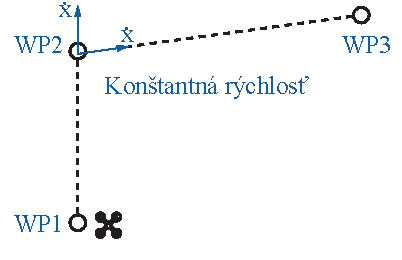
\includegraphics[width=60mm]{PositionControl2}\\
\end{figure}
\end{onlyenv}

\begin{onlyenv}<3>
  \begin{figure}
\centering
  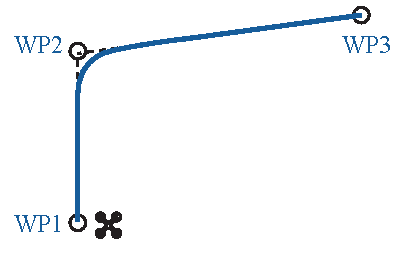
\includegraphics[width=60mm]{PositionControl3}\\
\end{figure}
\end{onlyenv}
\end{frame}
